% LaTeX example of generating a one-pager

% Standard document class set to landscape
\documentclass[a4paper]{article}


% Extra packages
\usepackage[hmargin=6mm,vmargin=10mm]{geometry}
\usepackage[usenames,dvipsnames]{color}
\usepackage{graphicx}
\usepackage{courier}
\usepackage{colortbl}


% Location of graphics
\graphicspath{{images/}}

% Define background colours for MMI levels
\definecolor{I}{RGB}{0,0,255}
\definecolor{II}{RGB}{32,159,255}
\definecolor{III}{RGB}{0,207,255}
\definecolor{IV}{RGB}{85,255,255}
\definecolor{V}{RGB}{170,255,255}
\definecolor{VI}{RGB}{255,240,0}
\definecolor{VII}{RGB}{255,168,0}
\definecolor{VIII}{RGB}{255,112,0}
\definecolor{IX}{RGB}{255,0,0}
\definecolor{X}{RGB}{240,0,240}

% Fixed with coloured cell
% Usage: \cell{color}{text}
\newcommand{\cell}[2]{
  \cellcolor{#1}
  \makebox[1.3cm]{#2}
}

% No page numbering
\pagestyle{empty}

% Begin document in earnest
\begin{document}

% Header
\begin{tabular}{lcr}

\includegraphics[width=0.08\textwidth]{bnpb_logo} &
\raisebox{10mm}{\parbox{0.75\textwidth}{\Huge \centerline{\textbf{Gempa Alert}}}} &

\includegraphics[width=0.08\textwidth]{bmkg_logo}
\end{tabular}

% Earthquake statistics as per BMKG sms
\bigskip
\begin{tabular}{@{}lr}
{\Large \textbf{Mag: 7.8 SR 29-Jan-11 23:40:20 WIB}} & \large Versi 1\\
{\Large \textbf{Lintang: 4.045$^\circ$ Garis bujur: 97.066$^\circ$ Kedalaman: 10.0km}}&\\
{\Large \textbf{115 km BaratDaya GUNUNGSITOLISUMUT}} &
\scriptsize Dibuat 36 minggu, 2 hari setelah gempa\\
\end{tabular}

% MMI legend
\bigskip
\begin{tabular}{|c|c|c|c|c|c|c|c|c|}
  \hline
  \multicolumn{9}{|c|}{\rule{0pt}{4mm} \Large \textbf{Estimasi penduduk terexpos pada tingkat getaran yang berbeda}} \\
   \hline
  \hline
  \textbf{Intensitas (MMI)} &
  \cell{II}{II} &
  \cell{III}{III} &
  \cell{IV}{IV} &
  \cell{V}{V} &
  \cell{VI}{VI} &
  \cell{VII}{VII} &
  \cell{VIII}{VIII} &
  \cell{IX}{IX}\\ \hline
  \textbf{Populasi} &
  0 & 6921 & 8864 & 1367 & 472 & 16 & 0 & 0 \\ \hline
  \textbf{Persepsi Gemetar} &
  Lemah & Lemah & Cahaya & Moderat & Kuat & Sangat Kuat & Parah & Keras   \\
  \noalign{\hrule height 0.6pt}
\end{tabular}

% Map elements
\bigskip
\begin{tabular}{l@{}l}
  \Large \textbf{Penduduk Paparan} & \\
  \parbox[t]{0.7\textwidth}{
    \vspace{0pt}
    \includegraphics{exposure_map}} &
  \parbox[t]{0.3\textwidth}{
    \vspace{0pt}
    \includegraphics[angle=270,width=0.25\textwidth]{city_legend} \\
    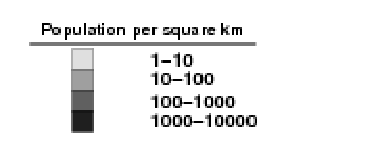
\includegraphics{population_legend}\\
    \includegraphics[width=0.25\textwidth]{mini_map}
  }
\end{tabular}


% PAGE 2
\clearpage
% Header
\begin{tabular}{lcr}

\includegraphics[width=0.08\textwidth]{bnpb_logo} &
\raisebox{10mm}{\parbox{0.75\textwidth}{\Huge \centerline{\textbf{Gempa Alert}}}} &

\includegraphics[width=0.08\textwidth]{bmkg_logo}
\end{tabular}

% Earthquake statistics as per BMKG sms
\bigskip
\begin{tabular}{@{}lr}
{\Large \textbf{Mag: 7.8 SR 29-Jan-11 23:40:20 WIB}} & \large Versi 1\\
{\Large \textbf{Lintang: 4.045$^\circ$ Garis bujur: 97.066$^\circ$ Kedalaman: 10.0km}}&\\
{\Large \textbf{115 km BaratDaya GUNUNGSITOLISUMUT}} &
\scriptsize Dibuat 36 minggu, 2 hari setelah gempa\\
\end{tabular}

% MMI legend
\bigskip
\includegraphics[angle=270,width=1.0\textwidth]{exposure_legend} \\

% Map elements
\bigskip
\begin{tabular}{l@{}l}
  \Large \textbf{Penduduk Paparan} & \\
  \parbox[t]{0.7\textwidth}{
    \vspace{0pt}
    \includegraphics{exposure_map}} &
  \parbox[t]{0.3\textwidth}{
    \vspace{0pt}
    \includegraphics[angle=270,width=0.25\textwidth]{city_legend} \\
    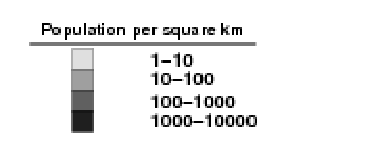
\includegraphics{population_legend}\\
    \includegraphics[width=0.25\textwidth]{mini_map}
  }
\end{tabular}


\end{document}


